\subsection{基于 SGX 的推测加密}
\label{subsec:encryption}

给定共享盲密钥 (\S\ref{subsec:key-management}),密钥安全区管理与每个客户端的安全通道,以在 MLE 密钥生成期间保护传输的指纹/密钥 (\S\ref{subsec:arch} )。然而,管理安全通道,特别是对于许多客户端,会在密钥安全区中产生高昂的加密/解密成本。 \sysname 在 SGX 的上下文中使用 {\em 推测加密} \cite{eduardo19} 增强了安全通信通道管理,从而减轻了密钥安全区的加密/解密开销。

\paragraph{推测加密} 推测加密 \cite{eduardo19} 采用{\em counter 模式} \cite{counter} 加解密,在离线过程中预先计算部分加解密结果,以减少在线独立加密文件系统中的计算开销。为了加密明文 $M$,我们首先将 $M$ 划分为一系列明文块 $b_1、b_2、\ldots、b_m$(例如,每个块的大小固定为 16 字节)。对于每个客户端,我们选择一个唯一的 {\em nonce} $\theta$,它只能被使用相同密钥的加密使用一次。然后我们计算第 $i$ 个明文块的 {\em 掩码}为 $e_i = {\bf E}(K, \theta || i)$,其中 ${\bf E}()$ 是对称加密函数,$K$ 是密钥,$i$ 是 {\em counter}(用于计数器模式加密),`$||$' 是连接运算符。最后,我们计算每个密文块$c_i = e_i \oplus b_i $,其中$\oplus$是按位异或运算符,并形成整个密文$C = c_1 || c_2 || \ldots || c_m$。为了解密密文,我们像上面一样为每个块生成掩码 $e_i$,恢复相应的明文块 $b_i = e_i \oplus c_i$ 并因此恢复原始明文 $M$。由于掩码生成步骤独立于每个目标明文/密文,我们可以离线预先计算掩码,然后应用轻量级 XOR 操作进行在线加密/解密。

\begin{figure}[t]
\centering
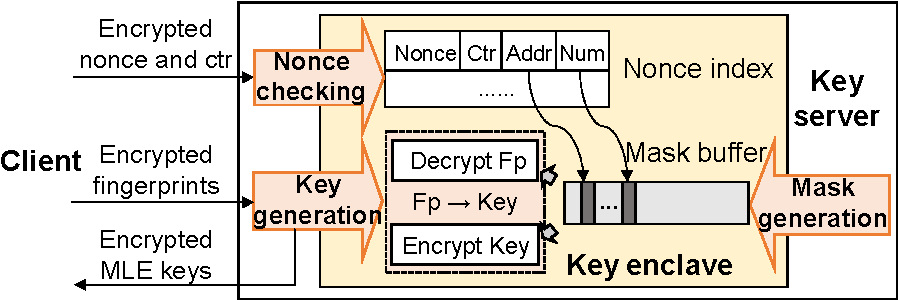
\includegraphics[width=3.3in]{pic/sgxdedup/encryption.pdf}
\caption{Overview of SGX-based speculative encryption.}
\label{fig:SpecEnc}
\end{figure}

\paragraph{Integration.} 要在 \sysname 中实现推测加密,我们需要解决 nonce、管理问题。、唯一的 nonce 充当不可预测的“一次性填充”,使得、每个 counter-mode 加密输出看起来随机 \cite{counter}。如果多个客户端使用反模式加密,我们需要在每个客户端的加密/解密操作中关联一个唯一的 nonce。但是,由于不同的客户端是隔离的,因此很难确保关联的 nonce客户是独一无二的。

为了确保 nonce 的唯一性,\sysname 在 key enclave 中管理一个集中的 key-value 存储,称为 {\em nonce index}。 nonce 索引的每个条目将存储的 nonce(12 字节)映射到三个字段:其计数器(4 字节)、相应掩码的起始地址(8 字节)和可用掩码的数量(4 字节)。此外,\sysname 实现了一个 {\em nonce checks ECall} (Figure~\ref{fig:SpecEnc}),它可以被密钥服务器调用,以将每个客户端提交的 nonce 与之前存储在 nonce 索引中的 nonce 进行比较,并如果发现重复的 nonce,通知客户重新选择一个新的。请注意,可以有效管理 in-enclave 随机数索引,因为它可以服务多达 112,000 个客户端(假设每个客户端一个随机数),只有 3MB EPC 空间(默认配置为 \sysname)。

\sysname 应用推测加密在客户端和密钥安全区之间建立安全通道,以保护 MLE 密钥生成。为了初始化安全通道,客户端将其自行选择的随机数 $\theta$ 和对应的计数器 $i$ 与密钥 enclave 同步,如果 $\theta$ 未用于任何加密,则 $i$ 初始化为零/由客户端解密。具体来说,它使用最新的盲密钥 (\S\ref{subsec:key-management}) 加密 $\theta$ 和 $i$,根据生成的密文计算消息验证码 (MAC),并将密文和 MAC 提交给密钥服务器。在这里,我们采用 {\em encrypt-then-MAC} \cite{bellare00} 通过检查 MAC 中的客户端和密钥安全区之间传输的任何信息来检测任何过时的盲密钥。

密钥服务器发出随机数检查 ECall,它将客户端的上传作为输入,解密 $\theta$ 和 $i$,并使用随机数索引检查解密后的 $\theta$ 和 $i$:
%
\begin{itemize}[leftmargin=*]
\item Case I:如果$\theta$ 是重复的并且$i$ = 0,这表示重复使用现有的nonce,并且ECall 返回一个信号通知客户端重新选择一个新的nonce。
\item 案例二:如果 $\theta$ 是重复的并且 $i \neq$ 为 0,这意味着 nonce 已被存储。 ECall 更新存储的计数器并标记相应的预计算掩码(用于后续处理,如下所述)。
\item 案例 III:如果 $\theta$ 是唯一的,这意味着 nonce 是新的,并且 ECall 将 $\theta$ 添加到 nonce 索引中。
\end{itemize}

对于 Cases~II 和 III,ECall 接受通信并要求客户端传输指纹以生成 MLE 密钥 (\S\ref{subsec:arch})。客户端根据$\theta$和$i$对指纹进行加密,并上​​传结果;在加密每个指纹块后,客户端将 $i$ 加一以防止重放攻击。如图~\ref{fig:SpecEnc}所示,密钥服务器发出{\em key generation ECall}来处理加密的指纹。 ECall 检查是否为当前客户端标记了某些掩码。如果找到(即情况 II),它使用标记的掩码来解密指纹并加密生成的 MLE 密钥。否则(即案例 III),它会在线计算掩码以进行解密和加密。

\paragraph{掩码预计算。} 为了加速加密/解密,当应用新的盲密钥(即所有现有掩码无效)或客户端在最后一个掩码后再次连接时,密钥安全区会执行掩码预计算代(即,它的一些掩码已被消耗)。关键安全区调用 {\em 掩码生成 ECall}(图~\ref{fig:SpecEnc}),它预先计算最近使用的随机数的数量(例如,在我们的例子中为三个)的掩码并写入将结果放入 {\em 掩码缓冲区}。默认情况下,我们将掩码缓冲区配置为最大 90\,MB。假设每个掩码占用 16 个字节,平均块大小为 8\,KB。指纹的 MLE 密钥生成使用四个掩码:两个用于解密 32 字节指纹,另外两个用于加密生成的 32 字节 MLE 密钥。因此,掩码缓冲区中预先计算的掩码可用于处理高达 11.25GB 数据的指纹。
